\documentclass[10pt,a4paper]{article}
\usepackage[T1]{fontenc}
\usepackage[utf8]{inputenc}
\usepackage{amssymb}
\usepackage{graphicx}
\usepackage[polish]{babel}
\usepackage{hyperref}
\usepackage[paper=a4paper,margin=1in]{geometry}
\usepackage{tabularx} 
\usepackage{helvet}
\usepackage{amsfonts}
\usepackage{amsthm}
\usepackage{mathtools}
\usepackage{algpseudocode}
\usepackage{tikz}
\usepackage{tkz-graph}
\usepackage{listings,xcolor}
\usepackage{scrextend}
\usepackage{float}
\usepackage{subcaption}
\renewcommand{\familydefault}{\sfdefault}
\setlength{\parindent}{0pt}
\newtheorem{definition}{Definicja}
\newtheorem{theorem}{Twierdzenie}
\newtheorem{lemma}{Lemat}
\newtheorem{invariant}{Niezmiennik}
\newtheorem{conculsion}{Wniosek}

\begin{document}
	\begin{titlepage}
		\newgeometry{top=1in,bottom=1in,right=1.5in,left=1.5in}
		\begin{center}
			{\fontsize{14}{12}\selectfont Politechnika Warszawska \\ Wydział Matematyki i Nauk Informacyjnych}
			
		\end{center}
		
		\vspace{1cm}
		\begin{center}
			
\includegraphics[width=0.3\textwidth]{images/logo.png}
		\end{center}
		\vspace{3cm}
		
		\begin{center}
			\textbf{{\fontsize{26}{12}\selectfont Chromatyczna Teoria Grafów}}
			
			\vspace{2cm}
			\textbf{{\fontsize{22}{12}\selectfont Dokumentacja projektowa}}
			\vspace{1cm}
			
			\textbf{{\fontsize{13.5}{12}\selectfont Chimedshirchin Batjargal, Mateusz Rymuszka}}
			
			\vspace{6cm}
			\textbf{{\fontsize{13.5}{12}\selectfont \today}}
		\end{center}  
	\end{titlepage}
	
	{\fontsize{13.5}{12}\selectfont
		\tableofcontents
		\vspace{1cm}
		{\renewcommand{\arraystretch}{2.0}
		\newpage
	}}
	
	\section{Abstrakt}
	
	Przedmiotem projektu realizowanego w ramach przedmiotu Chromatyczna Teoria Grafów przez autorów tego dokumentu jest analiza problemu kolorowania warstwowego grafu. Zespół przygotował, zaimplementował oraz przetestował działanie trzech algorytmów, które będą starały się pokolorować grafy wielowarstwowe w lepszy sposób niż naiwny algorytm duplikacji koloru na wiele warstw. W dokumentacji przedstawiono teoretyczny opis problemu wraz z proponowanymi algorytmami, a następnie sposób działania programu i raport z testów na wybranych rodzajach grafów, podsumowując to wszystko wnioskami płynącymi z obserwacji.
	
	\section{Opis teoretyczny problemu}
	
	\begin{definition}\label{def:1}
		\textbf{Kolorowaniem $p$-warstwowym} grafu $G$ nazywamy takie przyporządkowanie $c: v \rightarrow 2^{C}$, gdzie każdemu wierzchołkowi $v \in V(G)$ przypisujemy podzbiór $C'$ zbioru kolorów $C$ taki, że $|C'| = p$.
	\end{definition}

	\begin{definition}\label{def:2}
		Kolorowanie $p$-warstwowe grafu $G$ nazywamy \textbf{właściwym (poprawnym, optymalnym)}, jeżeli dla dowolnego $v \in V(G)$ przecięcia zbioru kolorów tego wierzchołka i kolorów każdego jego sąsiada są zbiorami pustymi, tzn.
		\[ \forall u, v \in V(G) \quad \left\{u, v\right\} \in E(G) \implies c(u) \cap c(v) = \emptyset \]
	\end{definition}

	Ogólnie rzecz ujmując, kolorowanie wielowarstwowe grafu jest rozszerzeniem zwykłego kolorowania grafu na wiele wymiarów. Kolorowanie jednowarstwowe jest tożsame z klasyczną definicją kolorowania wierzchołkowego grafu.
	
	\begin{definition}
		\textbf{$p$-warstwową liczbą chromatyczną} grafu $G$ nazywamy najmniejsze $q$ takie, że istnieje poprawne $p$-warstwowe pokolorowanie grafu $G$ używające $q$ kolorów.\\
		\textbf{Chromatycznym współczynnikiem $p$-warstwowym} grafu $G$ nazywamy stosunek $p$-warstwowej liczby chromatycznej do liczby warstw.
	\end{definition}

	Okazuje się, że $\chi_{p}G \leq p \chi G$. Gdy weźmiemy bowiem dobre $\chi G$-pokolorowanie $c: V \rightarrow C$ grafu $G$ i dla każdego $v \in V$ przypiszemy mu $c'(v) = \left\{r \cdot |C| + c(v): r \in \left\{1,...,p\right\}\right\}$, to uzyskamy $p \chi G$-pokolorowanie $p$-warstwowe. Nazwijmy je pokolorowaniem $p$-warstwowym grafu $G$ \textbf{równoległym do klasycznego}.
	\\~\\
	Przykładem grafu, który dla którego zachodzi ostra nierówność, jest nieparzysty cykl o wielkości przekraczającej trzy wierzchołki. Takie kolorowanie będziemy nazywać \textbf{lepszym od klasycznego}.
	
	\begin{figure}[H]
		\centering
		\begin{tikzpicture}
			\node[circle, draw, fill=none] (1) [label=south west:{1,2}] at (0,0) {};
			\node[circle, draw, fill=none] (2) [label=south east:{3,4}] at (4,0) {};
			\node[circle, draw, fill=none] (3) [label=south east:{5,1}] at (5,4) {};
			\node[circle, draw, fill=none] (4) [label=north:{2,3}] at (2,6) {};
			\node[circle, draw, fill=none] (5) [label=south west:{4,5}] at (-1,4) {};
			\draw (1) -- (2) -- (3) -- (4) -- (5) -- (1);
		\end{tikzpicture}
		\caption{Przykład 2,5-pokolorowania 2-warstwowego dla grafu $C_{5}$}
	\end{figure}
	
	Problem polega na znalezieniu takiego $p$-warstwowego pokolorowania dla zadanego $p$, aby dla pewnych grafów (takich, gdzie jest to możliwe) $\chi_{p}G < p \chi G$.
	
	\section{Proponowane algorytmy}
	
	Ponieważ problem znalezienia $p$-warstwowego grafu jest NP-trudny (można to wykazać, rozwijając graf warstwowo, gdzie każdy wierzchołek tworzy $p$-krotną klikę, zachowując połączenia z wierzchołkami w każdej z warstw), nie możemy znaleźć takiego pokolorowania w czasie wielomianowym. Zespół skupi się na poszukiwaniu algorytmu aproksymacyjnego, który przy zastosowaniu odpowiedniego podejścia do problemu, a być może pewnych heurystyk, będzie w stanie osiągać rezultat dla niektórych grafów.
	\\~\\
	Wspólnym mianownikiem tych algorytmów powinna być troska, aby starać się kolorować "chaotycznie", tzn. nie powtarzać tych samych zbiorów kolorów w wierzchołkach niezależnych. Taki układ może nas potem zmusić do użycia większej liczby kolorów, a w efekcie uzyskamy pokolorowanie na $p \cdot \chi G$ kolorów.
	
	\subsection{Zmodyfikowany algorytm AMIS}
	
	Algorytm AMIS (\textit{ang. approximately maximum independent set}) jest jednym z efektywniejszych algorytmów wielomianowych kolorowania grafu. W klasycznym problemie, polega on na wyborze spośród niepokolorowanych wierzchołków zbioru niezależnego i pokolorowanie go na nowy kolor. \\~\\
	Algorytm można byłoby zaaplikować bez większych zmian (dopóty wierzchołek uznajemy za niepokolorowany, dopóki nie posiada zbioru $p$ kolorów przypisanych do niego). Istnieje jednak ryzyko, że wybierając te same zbiory niezależne w kolejnych iteracjach algorytmu znajdowania zachłannego zbiorów niezależnych, uzyskalibyśmy pokolorowanie równoległe do klasycznego. Zależy nam zatem, aby w kolejnych iteracjach zbiory niezależne jednocześnie  nie były tożsame oraz nie były rozłączne. \\~\\
	Zaproponowany algorytm będzie korzystał ze zoptymalizowanej wersji algorytmu GIS (\textit{ang. greedy independent sets}), w którym zamiast wyboru wierzchołka na podstawie jego stopnia w grafie indukowanym, będziemy brali również pod uwagę częstość występowania danego wierzchołka w dotychczas wygenerowanych zbiorach niezależnych. 
	
	\subsubsection{Pseudokod}
	
	\begin{algorithmic}
		\State \textbf{Wejście:} graf $G$ i tablica wystąpień w zbiorach niezależnych wierzchołków $f$
		\\
		\Function {GreedyIndependentSet}{$G$, $f$}
			\State $G' \coloneqq G$
			\State $I \coloneqq \varnothing$
			\State less\_rank $\coloneqq true$
			\\
			\While{$V(G') > 0$}
				\State rank $\coloneqq$ [] 
				\ForAll{$v \in V(G')$}
				\State rank[$v$] $\coloneqq f(v) + \deg_{G'}(v)$ 
				\EndFor
				\\
				\If{less\_rank}
					\State $v = maxarg(\text{rank})$
				\Else
					\State $v = minarg(\text{rank})$
				\EndIf
				\State less\_rank $\coloneqq \neg$ less\_rank
				\\
				\State $I \coloneqq I \cup \left\{v\right\}$
				\State $G' = G'[V(G') - \left\{v\right\}- N_{G'}(v)]$
			\EndWhile
			\\
			\State \Return $I$
		\EndFunction
	\end{algorithmic}
	
	\begin{algorithmic}
		\State \textbf{Wejście:} graf $G$, liczba warstw $p$
		\\
		\Function {Color}{$G$, $p$}
			\State colored $\coloneqq 0$
			\State color $\coloneqq 1$
			\State $c \coloneqq \left[\right]$
			\State $f \coloneqq \left[\right]$
			\ForAll{$v \in V(G)$}
				\State $c(v) \coloneqq \varnothing$
				\State $f(v) \coloneqq 0$
			\EndFor
			\\
			\While{colored $< p \cdot |V(G)|$}
				\State $I \coloneqq $ \Call {GreedyIndependentSet}{$G\left[\left\{v \in V(G) : |c(v)| < p \right\}\right]$, $f$}
				\ForAll{$v \in I$}
					\State $c(v) \coloneqq c(v) \cup \left\{ \text{color} \right\}$
					\State $f(v) \coloneqq f(v) + 1$
					\State colored $\coloneqq$ colored $ + 1$
				\EndFor
			\EndWhile
			\State \Return $(\text{color}, c)$
		\EndFunction
	\end{algorithmic}

	\subsection{Zmodyfikowany algorytm DSATUR}
	
	Algorytm DSATUR należy do rodziny algorytmów sekwencyjnych. W klasycznym problemie, polega on na wyborze spośród niepokolorowanych wierzchołków zbioru niezależnego i pokolorowanie go na nowy kolor. Zespół postanowił nieco zmodyfikować ten algorytm i zbadać jego działanie dla problemu kolorowania wielowarstwowego.
	\\~\\
	Saturację w klasycznej wersji tego algorytmu traktowaliśmy jako liczbę unikalnych kolorów w sąsiednich pokolorowanych wierzchołkach. Aby algorytm działał dla wielu warstw, jednocześnie uwzględniając kolory znajdujące się u sąsiadów oraz w wierzchołku, należy zdefiniować nowy porządek. 
	\\~\\
	W celu analizy problemu, możemy rozpatrywać saturację wielorako; zdefiniujmy:
	\begin{itemize}
		\item saturację zewnętrzną, będącą ilością unikalnych kolorów użytych do pokolorowania wierzchołków sąsiednich, tzn.
		\[S^{OUT}_{G}(v) = \left|\bigcup_{u \in N_{G}(v)} c(u)\right|\]
		\item saturację wewnętrzną, będącą ilością kolorów użytych do pokolorowania wierzchołka, tzn.
		\[S^{IN}_{G}(v) = |c(v)|\]
		\item saturację całkowitą, będącą ilością unikalnych kolorów użytych do pokolorowania wierzchołków sąsiednich, tzn.
		\[S_{G}(v) = \left|\left(\bigcup_{u \in N_{G}(v)} c(u) \right) \cup c(v)\right|\]
	\end{itemize}
	Ponieważ $\forall u,v \in V(G) \quad {u, v} \in E(G) \implies c(u) \cap c(v) = \emptyset$ dla poprawnego $p$-warstwowego pokolorowania $c$ grafu $G$, mamy $S_{G}(v) = S^{OUT}_{G}(v) + S^{IN}_{G}(v)$. 
	\\~\\
	Rozpatrzymy dwa przypadki szeregowania wierzchołków na podstawie saturacji:
	\begin{itemize}
		\item wpierw malejąco po saturacji całkowitej, następnie rosnąco po saturacji wewnętrznej
		\item wpierw malejąco po saturacji zewnętrznej, następnie malejąco po saturacji wewnętrznej
	\end{itemize}

	\subsubsection{Pseudokod}

	\begin{algorithmic}
		\State \textbf{Wejście:} graf $G$, liczba warstw $p$, saturacja $S$
		\\
		\State colored $\coloneqq 0$
		\State max\_color $\coloneqq 0$ 
		\\
		\State $s_{in} \coloneqq \left[\right]$
		\State $s_{out} \coloneqq \left[\right]$
		\\
		\Procedure {ColorVertex}{$v$, \&$c$}
			\State color $\coloneqq 1$
			\While{color $\in s(v)$}
				\State color $\coloneqq$ color $+ 1$
			\EndWhile
			\\
			\State $c(v) = c(v) \cup \left\{\text{color}\right\}$
			\State colored $\coloneqq$ colored $ + 1$
			\If{color $>$ max\_color}
				\State max\_color $\coloneqq$ color
			\EndIf
			\\
			\State $s_{in}(v) = s_{in}(v) \cup \left\{\text{color}\right\}$
			\ForAll{$u \in N_{G}(v)$}
				\State $s_{out}(u) = s_{out}(u) \cup \left\{\text{color}\right\}$
			\EndFor
		\EndProcedure
		\newline
		\Function {Color}{$G$, $p$, $S$}
			\State $c \coloneqq \left[\right]$
			\\
			\ForAll{$v \in V(G)$}
				\State $c(v) = \varnothing$
				\State $s_{in}(v) = \varnothing$
				\State $s_{out}(v) = \varnothing$
			\EndFor
			\\
			\State $v \coloneqq rand(\left\{v \in V(G): \forall u \in V(G) \deg_{G} v \geq \deg_{G} u \right\})$
			\State \Call {ColorVertex}{$v$, \&$c$, \&$s$}
			\\
			\While{colored $< p \cdot |V(G)|$}
				\State $v \coloneqq rand(\left\{v \in V(G): \forall u \in V(G) S(v) \geq S(u) \right\})$
				\State \Call {ColorVertex}{$v$, \&$c$, \&$s$}
			\EndWhile
			\\
			\State \Return $(\text{max\_color}, c)$
		\EndFunction
	\end{algorithmic}

	\subsection{Zmodyfikowany algorytm CS}
	
	Ostatnim algorytmem zaproponowanym przez zespół będzie zmodyfikowany algorytm podobny do algorytmu CS (\textit{ang. connected sequential}). Jego modyfikacja będzie polegała na tym, że w przypadku konieczności użycia koloru, zostanie uruchomiona procedura wymiany, bazująca na algorytmie wyznaczania permutacji Fishera-Yatesa. Algorytm zakłada, że w przypadku braku dostępnego koloru z puli, będziemy po kolei iść wzdłuż pewnej ścieżki od naszego wierzchołka i próbować wymieniać kolory do momentu, gdy któryś z wierzchołków będzie się dało pokolorować użytymi już kolorami, albo gdy algorytm zakończy permutację. Nowego koloru użyjemy tylko w drugim przypadku. Aby zwiększyć skuteczność, będziemy sprawdzać wymianę wszystkich możliwych kolorów.
	
	\subsubsection{Pseudokod}
	
	\begin{algorithmic}
		\State \textbf{Wejście:} graf $G$, liczba warstw $p$ \\
		\State colored $\coloneqq 0$
		\State max\_color $\coloneqq 0$
		\\
		\Procedure {ColorInterchange}{$v$, \&$G$, \&$c$}
			\State $A \coloneqq \varnothing$
			\\
			\For{$i \coloneqq 1$; $i \leq V(G)$; ++$i$}
				\State $u \coloneqq rand(\left\{u \in N_{G}(v) - A : c(u) - c[N_{G}(v) \cup \left\{v\right\} - \left\{u\right\}] \neq \varnothing \right\})$
				\State $A \coloneqq A \cup \left\{u\right\}$
				\\
				\ForAll{$x \in c(u) - c[N_{G}(v) \cup \left\{v\right\} - \left\{u\right\}]$}
					\State $c(u) \coloneqq c(u) - \left\{x\right\}$
					\State $c(v) \coloneqq c(v) \cup \left\{x\right\}$
					\\
					\ForAll{$y \in \left\{1, ..., \text{max\_color}\right\}$}
						\If{$y \notin c\left[N_{G}(u) \cup \left\{u\right\}\right]$}
							\State $c(u) \coloneqq c(u) \cup \left\{y\right\}$
							\State \Return $true$
						\EndIf
					\EndFor
					\\
					\State $c(u) \coloneqq c(u) \cup \left\{x\right\}$
					\State $c(v) \coloneqq c(v) - \left\{x\right\}$
				\EndFor
				\\
				\State $x = rand(c(u) - c[N_{G}(v) \cup \left\{v\right\} - \left\{u\right\}])$
				\State $c(u) \coloneqq c(u) - \left\{x\right\}$
				\State $c(v) \coloneqq c(v) \cup \left\{x\right\}$
				\\
				\State $v \coloneqq u$
			\EndFor
			\State \Return $false$
		\EndProcedure
		\\
		\Function {Color}{$G$, $p$}
			\State $c \coloneqq \left[\right]$
			\ForAll{$v \in V(G)$}
				\State $c(v) = \varnothing$
			\EndFor
			\\
			\ForAll{$v \in V(G)$, $l \in \left\{1,...,p\right\}$}
				\ForAll{color $\in \left\{1,...,\text{max\_color}\right\}$}
					\If{color $\notin c\left[\left\{v\right\} \cup N_{G}(v) \right]$}
						\State $c(v) \coloneqq c(v) \cup \left\{\text{color}\right\}$
						\State \textbf{break}
					\EndIf
				\EndFor
				\If{$\neg$\Call {ColorInterchange}{$v$, \&$G$, \&$c$}}
					\State $c(v) \coloneqq c(v) \cup \left\{\text{color} + 1\right\}$
					\State max\_color $\coloneqq$ max\_color $+ 1$
				\EndIf
			\EndFor
			\State \Return $(c, \text{max\_color})$
		\EndFunction
	\end{algorithmic}	
	
	\section{Założenia techniczne}
	
	W wyborze języka, w którym zostanie stworzony program, zespół kierował się przejrzystością implementacji, aby móc skupić się na teoretycznej części problemu. Ostatecznie, program został napisany w języku Python. Jest to język wieloparadygmatowy o wyjątkowo prostej składni, co pozwala w dość obrazowy sposób przedstawić istotę zaproponowanych algorytmów. Dodatkowo, posiada duże wsparcie społeczności. 
	\\~\\
	Projekt będzie obejmował:
	\begin{itemize}
		\item interfejs użytkownika (parser wejścia, komunikaty itp.)
		\item implementację wyżej wymienionych algorytmów 
		\item prezentację wyniku (wyjście tekstowe)
		\item przykładowe benchmarki testujące skuteczność oraz czas wykonania na wybranych grafach
	\end{itemize}

	\section{Zmiany w stosunku do dokumentacji początkowej}
	
	Zespół zdecydował się na zmianę strategii w niektórych algorytmach, ze względu na napotkane trudności implementacyjne:
	\begin{enumerate}
		\item w algorytmie AMIS losowe generowanie wierzchołków i późniejsze usuwanie ich ze zbioru wierzchołków niezależnych, ze względu na brak czynnika wyróżniającego niezbędną kolejność usuwania wierzchołków, może prowadzić do generowania małych zbiorów niezależnych; z tego powodu zdecydowano się wybór jednego wierzchołka, przy zachowaniu parametru częstości występowania w zbiorach niezależnych
		\item do algorytmu DSATUR, poza wyborem wierzchołka na podstawie saturacji całkowitej z preferencją dla wierzchołków o mniejszej saturacji wewnętrznej, dodano wybór wierzchołka na podstawie saturacji zewnętrznej z preferencją dla wierzchołków o większej saturacji wewnętrznej
		\item algorytm Connected Sequential z wymianą wierzchołków będzie starał się przeszukiwać najdłuższą możliwą ścieżkę, aby zwiększyć szansę na wymianę kolorów; dodatkowo, algorytm będzie analizował wszystkich tych sąsiadów, którzy są w stanie wymienić się kolorami (przynajmniej jednym) z aktualnym wierzchołkiem i wybierał losowo spośród nich, a nie wszystkich sąsiadów - ma to uniknąć częstym sytuacjom, gdy wybrany sąsiad nie ma koloru do wymiany
	\end{enumerate}
	
	Ponadto, ostatecznie zespół zdecydował się na implementację algorytmów i testów w języku Python - ze względu na większą prostotę, elastyczność oraz łatwość tworzenia testów i rysowania wykresów obrazujących wyniki eksperymentów. Ze względu na rozmiar badanych grafów, zrezygnowano również z prezentacji wizualnej kolorowania.

	\section{Opis struktury projektu}
	
	Projekt będzie składał się z dwóch modułów:
	\begin{itemize}
		\item moduł implementacyjny \texttt{coloring} - zostały w nim zawarte:
			\begin{itemize}
				\item implementacja struktura grafu, oparta o słownik sąsiadów (plik \texttt{graph.py}),
				\item implementacja algorytmów kolorowania warstwowego (plik \texttt{coloring.py}),
				\item moduł generujący przykładowe instancje lub ładujący przykłady z pliku w formie DIMACS (plik \texttt{examples.py})
			\end{itemize}
		\item moduł testów \texttt{test} - zostały w nim zawarte pliki opisujące przeprowadzone testy wydajności i efektywności zaimplementowanych algorytmów
		\item plik \texttt{run.py} - umożliwia uruchomienie jednego lub wszystkich algorytmów na wybranym grafie (w formie pliku DIMACS, podanym jako argument); skrypt zwróci czas potrzebny na wykonanie obliczeń, liczbę kolorów użytych oraz chromatyczny współczynnik otrzymanego pokolorowania, a także wypisze lub zapisze kolorowanie do pliku 
	\end{itemize}

	\pagebreak
	
	\section{Raport z przeprowadzonych testów i eksperymentów}
	
	\subsection{Wprowadzenie}
	
	W trakcie testów zespół starał się ująć istotę problemu w postaci uzyskania chromatycznego współczynnika warstwowego na poziomie niższym niż liczba chromatyczna danego grafu (tzn. uzyskania lepszego pokolorowania niż klasyczne). Z tego powodu dużą rolę w testach pełni odpowiedni dobór grafów wykorzystywanych do testów. 
	\\~\\
	W testach uwzględniliśmy cztery klasy grafów:
	\begin{itemize}
		\item cykle nieparzyste - są to najmniejsze grafy, których warstwowe pokolorowania są lepsze od klasycznych; testy na tych grafach będą służyły jako najprostsze testy skuteczności
		\item grafy Knesera - w szczególności grafy Petersena - ich złożona struktura oraz znana liczba chromatyczna (dla grafu $K(k, n)$ wynosi ona $n - 2k + 2$) pozwolą na przetestowanie skuteczności dla nieco bardziej złożonych grafów niż nieparzyste cykle
		\item wybrane przykłady ze zbioru grafów trudnych do kolorowania ze strony prowadzącego przedmiot \cite{gci}
	\end{itemize}
	Grafy będą testowane pod kątem skuteczności (tzn. współczynnikowi chromatycznemu dla danej ilości warstw) oraz szybkości algorytmu w porównaniu do innych.
	
	\subsection{Testy na nieparzystych cyklach}
	
	Pierwszą grupą grafów, dla których zostały przeprowadzone testy, są nieparzyste cykle. Są to najmniejsze grafy, dla których można zaobserwować lepsze $p$-warstwowe pokolorwania dla $p > 1$ - sprzyjają one zatem początkowej analizie problemu oraz oszacowaniu ewentualnych możliwości naszych algorytmów.
	\\~\\
	Testy zostały przeprowadzone na cyklach o różnej długości oraz przy zastosowaniu algorytmu dla wielu warstw. Przy testowaniu wydajności algorytmu względem długości cyklu sprawdzaliśmy cykle o długościach od $5$ do $75$ (z krokiem $10$) oraz ilościach warstw: $2$, $3$, $5$ oraz $10$. Podobnie wyglądały testy ze względu na ilość warstw, lecz tutaj ograniczyliśmy się do cykli o długościach od $5$ do $45$ z $10$. Te same wyniki zastosowaliśmy później do oceny efektywności naszych algorytmów.
	\\~\\
	Wnioski płynące z obserwacji pozwalają nam stwierdzić, że dla krótszych cykli zdecydowanie szybciej działają algorytmu z klasy DSATUR. W miarę wzrostu długości cyklu, długości ich wykonywania wzrasta w porównaniu do pozostałych algorytmów. W ten sposób algorytm CS z wymianą wierzchołków, który na początku był jednym z najdłużej działających algorytmów, staje się jednym z najszybszych. 
	\\~\\
	Ilość warstw ma znaczny wpływ na działanie wszystkich algorytmów dla cykli nieparzystych. O ile w przypadku algorytmów AMIS czy DSATUR charakterystyka przypomina liniowy lub nadliniowy trend wzrostu, algorytm CS z wymianą zdecydowanie wzrasta w tempie co najmniej kwadratowym. Widzimy jednak, że im dłuższy cykl, tym mniejsze różnice w czasie wykonania między poszczególnymi algorytmami.
	\\~\\
	W przypadku oceny efektywności algorytmów, w każdym przypadku cykle dawały tę samą liczbę kolorów dla danej długości grafu oraz danej ilości warstw (dane na 100 przebiegów). Można jednak zauważyć, że dla algorytmów z klasy DSATUR osiągany współczynnik chromatyczny był równy liczbie chromatycznej, czyniąc ten algorytm najsłabszym do zastosowania dla nieparzystych cykli. Dość dobrze radził sobie algorytm AMIS, który w większości zadanych konfiguracji osiągał współczynnik niższy od liczby chromatycznej, od $2.5$ do $3$. Zdecydowanie lepiej sobie radził dla większych ilości warstw. Najlepszym algorytmem okazał się tutaj algorytm CS z wymianą - był on w stanie osiągać nawet współczynniki na poziomie $2.1$ dla dziesięciu warstw oraz cykli dłuższych od $5$. 
	
	\pagebreak
	
	\vspace*{\fill}
	\begin{figure}[H]
		\begin{center}
			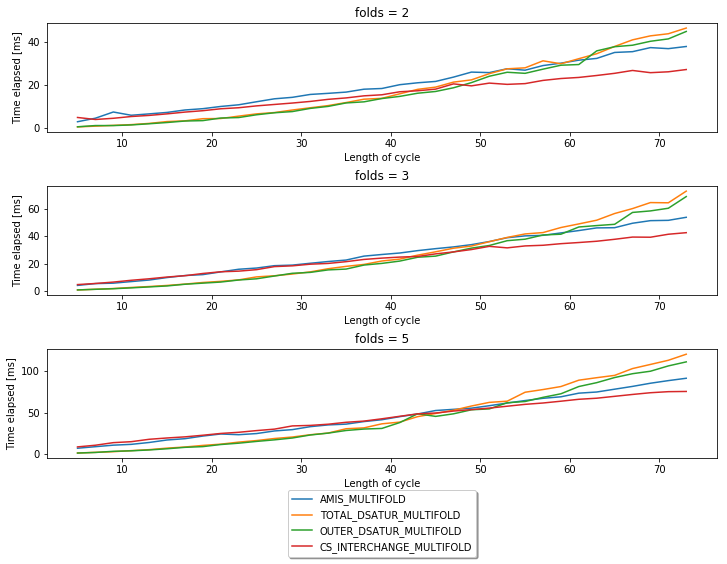
\includegraphics[width=\textwidth]{images/tests/odd_cycles/performance_per_cycle_length.png}
			\caption{Wykres zależności długości cyklu od czasu wykonania algorytmu dla wybranych ilości warstw}
		\end{center}
	\end{figure}
	\vspace*{\fill}
	
	\pagebreak

	\vspace*{\fill}
	\begin{figure}[H]
		\begin{center}
			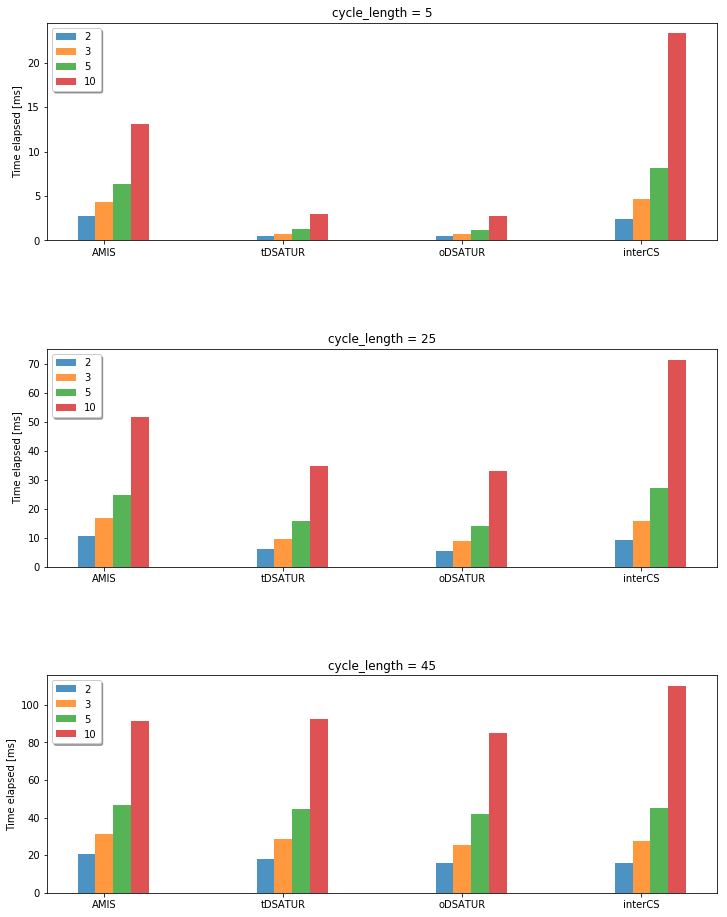
\includegraphics[width=\textwidth]{images/tests/odd_cycles/performance_per_folds.png}
			\caption{Wykres zależności ilości warstw od czasu wykonania algorytmu dla wybranych długości cyklu}
		\end{center}
	\end{figure}
	\vspace*{\fill}
	
	\pagebreak
	
	\begin{table}[H]
		\centering
		\begin{tabular}{|l|l|c|c|c|c|}
			\hline
			\textbf{warstwy} & \textbf{długość cyklu} & \textbf{AMIS} & \textbf{total DSATUR} & \textbf{outer DSATUR} & \textbf{interchange CS} \\		
			\hline
			2 & 5 & 2.5 & 3.0 & 3.0 & 2.5 \\ 
			3 & 5 & 2.67 & 3.0 & 3.0 & 2.67 \\ 
			5 & 5 & 2.8 & 3.0 & 3.0 & 2.6 \\ 
			10 & 5 & 2.6 & 3.0 & 3.0 & 2.5 \\ 
			\hline
			2 & 15 & 3.0 & 3.0 & 3.0 & 2.5 \\ 
			3 & 15 & 2.67 & 3.0 & 3.0 & 2.33 \\ 
			5 & 15 & 2.6 & 3.0 & 3.0 & 2.2 \\ 
			10 & 15 & 2.6 & 3.0 & 3.0 & 2.2 \\ 
			\hline
			2 & 25 & 3.0 & 3.0 & 3.0 & 2.5 \\ 
			3 & 25 & 3.0 & 3.0 & 3.0 & 2.33 \\ 
			5 & 25 & 2.8 & 3.0 & 3.0 & 2.2 \\ 
			10 & 25 & 2.7 & 3.0 & 3.0 & 2.1 \\ 
			\hline
			2 & 35 & 3.0 & 3.0 & 3.0 & 2.5 \\ 
			3 & 35 & 3.0 & 3.0 & 3.0 & 2.33 \\ 
			5 & 35 & 2.8 & 3.0 & 3.0 & 2.2 \\ 
			10 & 35 & 2.8 & 3.0 & 3.0 & 2.1 \\ 
			\hline
			2 & 45 & 3.0 & 3.0 & 3.0 & 2.5 \\ 
			3 & 45 & 3.0 & 3.0 & 3.0 & 2.33 \\ 
			5 & 45 & 2.8 & 3.0 & 3.0 & 2.2 \\ 
			10 & 45 & 2.7 & 3.0 & 3.0 & 2.1 \\
			\hline
		\end{tabular}
		\caption{Współczynnik $p$-warstwowego kolorowania uzyskanego dla grafów }
	\end{table}

	
	Widzimy, że w przypadku cykli nieparzystych algorytmy były dość odporne na losowości - wynikało to z prostej propagacji algorytmu zgodnie/przeciwnie do ruchu wskazówek zegara. W związku z tym wyniki dość jednoznacznie określiły, który algorytm nadaje się do aplikacji do tej klasy grafów. W dalszej analizie sprawdzimy, jakie rezultaty zostały osiągnięte na innych, bardziej skomplikowanych grafach.
	
	\subsection{Testy na grafach Knesera}
	
	Kolejną grupą grafów, które zostały poddane testom, są grafy Knesera. Są to grafy postaci $K(n, k)$, gdzie:
	\begin{itemize}
		\item wierzchołki grafu $K(n, k)$ są etykietowane podzbiorami $k$-elementowymi zbioru $n$-elementowego.
		\item dwa wierzchołki są połączone krawędzią wtedy i tylko wtedy, gdy zbiory będące etykietami tychże wierzchołków są rozłączne
	\end{itemize}

	Grafy Knesera mogą stanowić interesujący obiekt badawczy z tego względu, że w przypadku rozpatrywania pokolorowania $k$-warstwowego, wprost z definicji wynika fakt, że współczynnik chromatyczny takiego grafu powinien wynosić $\frac{n}{k}$. Różne rezultaty może być też badanie skuteczności algorytmów dla innej liczby warstw niż $k$. Liczba chromatyczna grafu Knesera $K(n,k)$ wynosi dla zaprezentowanych przykładów $n - 2k + 2$.
	\\~\\
	W pierwszej kolejności została zbadana wydajność badanych algorytmów na grafach Knesera. Z przedstawionych poniżej wykresów możemy łatwo ocenić, iż najbardziej czasochłonnym jest algorytm CS z wymianą. Jego tempo wzrostu jest ściśle skorelowane, podobnie jak w przypadku nieparzystych cykli, z liczbą warstw. Algorytm AMIS jest drugim od końca pod względem szybkości w przypadku wszystkich grafów, wyłączając $K(9, 4)$. Najszybsze są algorytmy DSATUR, z lekką przewagą algorytm z wyborem wierzchołka o największej saturacji zewnętrznej, jednak dla $K(9, 4)$ najszybszy jest AMIS, który wyprzedza te dwa algorytmy. 
	\\~\\
	Efektywność algorytmu AMIS dla większych grafów Knesera wynika zapewne z faktu, że posiadają one na tyle liczne zbiory niezależne, że narzut czasowy wynikający z konieczności analizy każdego wierzchołka w algorytmie DSATUR zaczyna przeważać nad czasem znalezienia zbioru niezależnego w grafie, który posiada dość liczną rodzinę zbiorów niezależnych. 
	
	\pagebreak
	
	\vspace*{\fill}
	\begin{figure}[H]
		\begin{center}
			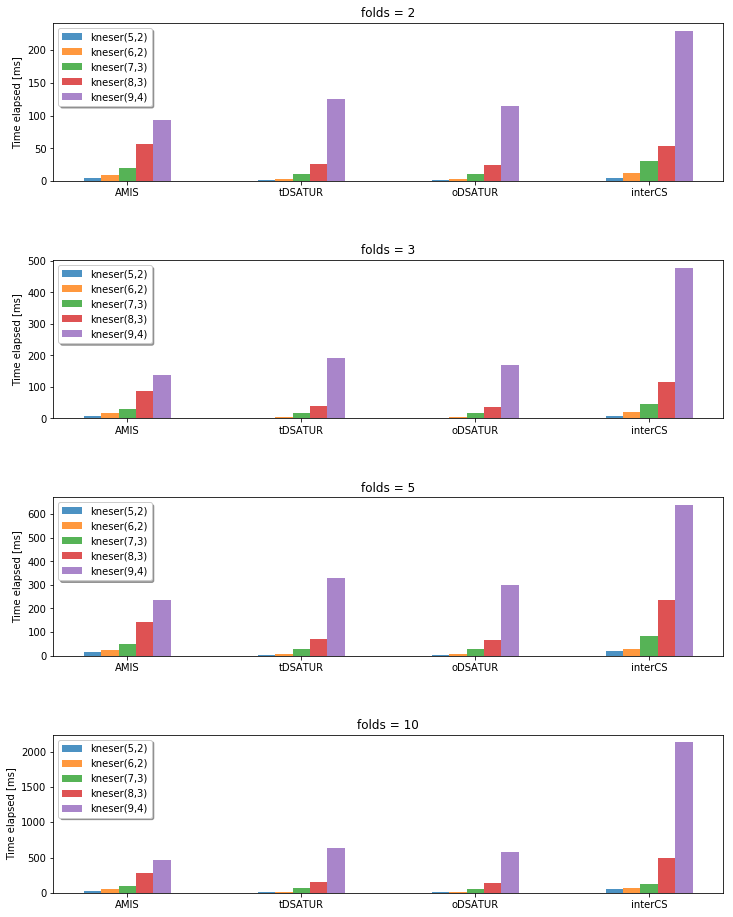
\includegraphics[width=\textwidth]{images/tests/kneser_graphs/performance_per_graph.png}
			\caption{Porównanie czasu wykonania algorytmów na grafach Knesera dla wybranych grafów}
		\end{center}
	\end{figure}
	\vspace*{\fill}
	
	\pagebreak
	
	\vspace*{\fill}
	\begin{figure}[H]
		\begin{center}
			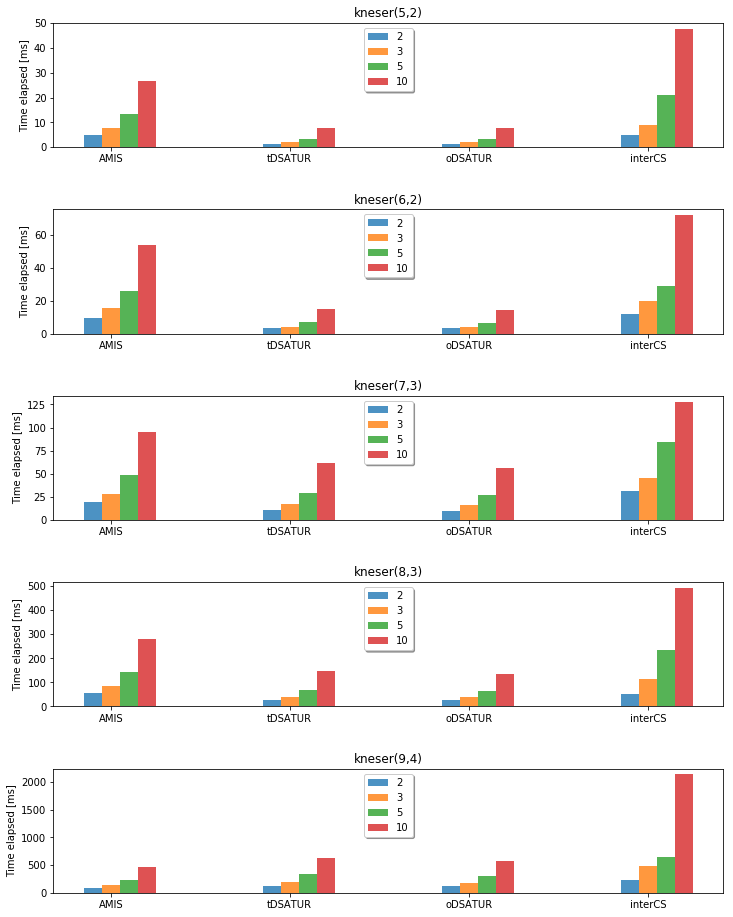
\includegraphics[width=\textwidth]{images/tests/kneser_graphs/performance_per_folds.png}
			\caption{Porównanie czasu wykonania algorytmu na grafach Knesera dla wybranych ilości warstw}
		\end{center}
	\end{figure}
	\vspace*{\fill}
	
	\pagebreak

	\begin{table}[H]
		\begin{minipage}{.5\linewidth}
			\centering
			\begin{tabular}{|l|c|c|c|c|}
				\hline
				\textbf{$p$} & \textbf{algorytm} & \textbf{$\min \chi_{p}$} & \textbf{$|\min \chi_{p}|$} & \textbf{$\overline{\chi_{p}}$} \\
				\hline
				2 & AMIS & 2.5 & 100 & 2.5 \\
				2 & interCS & 2.5 & 25 & 2.88 \\
				2 & oDSATUR & 3.0 & 100 & 3.0 \\
				2 & tDSATUR & 3.0 & 100 & 3.0 \\
				\hline
				3 & AMIS & 2.67 & 100 & 2.67 \\
				3 & interCS & 2.67 & 57 & 2.81 \\
				3 & oDSATUR & 3.0 & 100 & 3.0 \\
				3 & tDSATUR & 3.0 & 98 & 3.01 \\
				\hline
				5 & AMIS & 3.0 & 100 & 3.0 \\
				5 & interCS & 3.0 & 100 & 3.0 \\
				5 & oDSATUR & 3.0 & 100 & 3.0 \\
				5 & tDSATUR & 3.0 & 100 & 3.0 \\
				\hline
				10 & AMIS & 3.0 & 100 & 3.0 \\
				10 & interCS & 2.5 & 3 & 2.66 \\
				10 & oDSATUR & 3.0 & 98 & 3.0 \\
				10 & tDSATUR & 3.0 & 100 & 3.0 \\
				\hline
			\end{tabular}
			\caption{$K(5,2)$}
		\end{minipage}%
		\begin{minipage}{.5\linewidth}
			\centering
			\begin{tabular}{|l|c|c|c|c|}
				\hline
				\textbf{$p$} & \textbf{algorytm} & \textbf{$\min \chi_{p}$} & \textbf{$|\min \chi_{p}|$} & \textbf{$\overline{\chi_{p}}$} \\
				\hline
				2 & AMIS & 3.0 & 100 & 3.0 \\
				2 & interCS & 3.5 & 100 & 3.5 \\
				2 & oDSATUR & 3.0 & 52 & 3.48 \\
				2 & tDSATUR & 3.0 & 55 & 3.45 \\
				\hline
				3 & AMIS & 3.33 & 100 & 3.33 \\
				3 & interCS & 4.0 & 100 & 4.0 \\
				3 & oDSATUR & 3.33 & 78 & 3.48 \\
				3 & tDSATUR & 3.33 & 96 & 3.36 \\
				\hline
				5 & AMIS & 3.8 & 100 & 3.8 \\
				5 & interCS & 3.4 & 88 & 3.43 \\
				5 & oDSATUR & 3.2 & 69 & 3.34 \\
				5 & tDSATUR & 3.2 & 84 & 3.28 \\
				\hline
				10 & AMIS & 3.7 & 100 & 3.7 \\
				10 & interCS & 3.0 & 100 & 3.0 \\
				10 & oDSATUR & 3.0 & 19 & 3.24 \\
				10 & tDSATUR & 3.0 & 2 & 3.24 \\
				\hline
			\end{tabular}
			\caption{$K(6,2)$}
		\end{minipage} 
		\begin{minipage}{.5\linewidth}
			\centering
			\begin{tabular}{|l|c|c|c|c|}
				\hline
				\textbf{$p$} & \textbf{algorytm} & \textbf{$\min \chi_{p}$} & \textbf{$|\min \chi_{p}|$} & \textbf{$\overline{\chi_{p}}$} \\
				\hline
				2 & AMIS & 3.5 & 100 & 3.5 \\
				2 & interCS & 2.5 & 6 & 3.06 \\
				2 & oDSATUR & 3.0 & 95 & 3.02 \\
				2 & tDSATUR & 3.0 & 89 & 3.06 \\
				\hline
				3 & AMIS & 3.67 & 100 & 3.67 \\
				3 & interCS & 3.0 & 100 & 3.0 \\
				3 & oDSATUR & 3.0 & 91 & 3.04 \\
				3 & tDSATUR & 3.0 & 78 & 3.08 \\
				\hline
				5 & AMIS & 3.4 & 100 & 3.4 \\
				5 & interCS & 2.6 & 3 & 2.87 \\
				5 & oDSATUR & 3.0 & 80 & 3.05 \\
				5 & tDSATUR & 3.0 & 74 & 3.07 \\
				\hline
				10 & AMIS & 3.3 & 100 & 3.3 \\
				10 & interCS & 2.7 & 10 & 2.84 \\
				10 & oDSATUR & 3.0 & 73 & 3.05 \\
				10 & tDSATUR & 3.0 & 74 & 3.06 \\
				\hline
			\end{tabular}
			\caption{$K(7,3)$}
		\end{minipage}%
		\begin{minipage}{.5\linewidth}
			\centering
			\begin{tabular}{|l|c|c|c|c|}
				\hline
				\textbf{$p$} & \textbf{algorytm} & \textbf{$\min \chi_{p}$} & \textbf{$|\min \chi_{p}|$} & \textbf{$\overline{\chi_{p}}$} \\
				\hline
				2 & AMIS & 6.0 & 100 & 6.0 \\
				2 & interCS & 3.5 & 10 & 4.04 \\
				2 & oDSATUR & 3.0 & 1 & 4.08 \\
				2 & tDSATUR & 3.0 & 4 & 4.11 \\
				\hline
				3 & AMIS & 5.67 & 100 & 5.67 \\
				3 & interCS & 3.33 & 2 & 3.81 \\
				3 & oDSATUR & 3.0 & 5 & 3.85 \\
				3 & tDSATUR & 3.33 & 1 & 4.14 \\
				\hline
				5 & AMIS & 5.8 & 100 & 5.8 \\
				5 & interCS & 3.2 & 7 & 3.56 \\
				5 & oDSATUR & 3.0 & 1 & 3.74 \\
				5 & tDSATUR & 3.4 & 1 & 4.13 \\
				\hline
				10 & AMIS & 5.1 & 100 & 5.1 \\
				10 & interCS & 4.0 & 34 & 4.11 \\
				10 & oDSATUR & 3.0 & 4 & 3.76 \\
				10 & tDSATUR & 3.1 & 1 & 4.08 \\
				\hline
			\end{tabular}
			\caption{$K(8,3)$}
		\end{minipage}
		\hspace{55pt}
		\begin{minipage}{\linewidth}
			\centering
			\begin{tabular}{|l|c|c|c|c|}
				\hline
				\textbf{$p$} & \textbf{algorytm} & \textbf{$\min \chi_{p}$} & \textbf{$|\min \chi_{p}|$} & \textbf{$\overline{\chi_{p}}$} \\
				\hline
				2 & AMIS & 4.5 & 100 & 4.5 \\
				2 & interCS & 3.0 & 6 & 3.53 \\
				2 & oDSATUR & 3.0 & 64 & 3.18 \\
				2 & tDSATUR & 3.0 & 49 & 3.26 \\
				\hline
				3 & AMIS & 4.33 & 100 & 4.33 \\
				3 & interCS & 3.33 & 18 & 3.66 \\
				3 & oDSATUR & 3.0 & 56 & 3.16 \\
				3 & tDSATUR & 3.0 & 39 & 3.21 \\
				\hline
				5 & AMIS & 4.4 & 100 & 4.4 \\
				5 & interCS & 3.0 & 11 & 3.27 \\
				5 & oDSATUR & 3.0 & 52 & 3.12 \\
				5 & tDSATUR & 3.0 & 21 & 3.23 \\
				\hline
				10 & AMIS & 3.9 & 100 & 3.9 \\
				10 & interCS & 3.1 & 3 & 3.33 \\
				10 & oDSATUR & 3.0 & 33 & 3.11 \\
				10 & tDSATUR & 3.0 & 26 & 3.18 \\
				\hline
			\end{tabular}
			\caption{$K(9,4)$}
		\end{minipage}
		\caption{Porównanie współczynników chromatycznych osiąganych przez testowane algorytmy na grafach Knesera dla wybranych ilości warstw }
	\end{table}

	Wyniki efektywności badanych algorytmów na grafach Knesera ukazują dość ciekawe rezultaty. W przypadku grafu Petersena $K(5,2)$ jedynie algorytmom DSATUR nie udało się osiągnąć lepszego współczynnika od liczby chromatycznej dla żadnej ilości warstw. Algorytm AMIS miał dobrą skuteczność dla $p = 2$ i $p = 3$, lecz dla większej ilości warstw nadal pozostawał na poziomie pokolorowania klasycznego. Z kolei algorytm interCS osiągał w pewnej liczbie przypadków niższy współczynnik nawet dla większej ilości warstw (wyłączając liczbę warstw $p = 5$, kiedy to każdy algorytm miał pokolorowanie równe klasycznemu). 
	\\~\\
	W przypadku grafów $K(6,2)$ i $K(8,3)$ osiągnięto dość dobre rezultaty - ich liczba chromatyczna wynosi $4$, lecz poza algorytmem AMIS wszystkim algorytmom udało się znaleźć pokolorowania warstwowe lepsze od klasycznego. Nieco lepiej działały one dla $K(6, 2)$, kiedy odsetek tych pokolorowań był większy, a średni współczynnik na ogół był niższy od liczby chromatycznej. Graf $K(8, 2)$ też miewał lepsze pokolorowania, lecz były one znacznie rzadsze niż w poprzednim wypadku. Widać także różnicę w skuteczności poszczególnych algorytmów - dla algorytmu interCS pokolorowania lepsze zdarzały się częściej niż dla algorytmów DSATUR, chociaż nie była to istotna różnica. 
	\\~\\
	W przypadku grafów $K(7,3)$ i $K(9,4)$ rezultaty są dość słabe - nie dość, że nie udawało się na ogół uzyskać lepszych pokolorowań (poza kilkoma przypadkami dla algorytmu interCS), to jeszcze często osiągano gorsze wyniki od pokolorowania klasycznego. Tutaj także widać słabość algorytmu AMIS, który nie nadaje się do optymalnego kolorowania warstwowego dla większych grafów Knesera.
	
	\subsection{Testy na grafach hetmańskich}
	
	Graf hetmański $Q(n)$ jest grafem reprezentujący problem $n$ hetmanów - posiada on $n^{2}$ wierzchołków, które odpowiadają polom na szachownicy $n \times n$. Wierzchołki są połączone krawędzią wtedy i tylko wtedy, gdy znajdują się w jednym rzędzie, kolumnie lub są na jednej diagonali (czyli odpowiadają zasięgowi hetmana).
	\\~\\
	Dla niektórych ta liczba nie jest znana, lecz niektóre grafy mają znane liczby chromatyczne:
	\begin{itemize}
		\item $Q(5)$ - $5$
		\item $Q(6)$ - $7$
		\item $Q(7)$ - $7$
		\item $Q(8)$ - $8$
		\item $Q(9)$ - $9$
		\item $Q(11)$ - $11$
		\item $Q(13)$ - $13$
	\end{itemize}
	W tej sekcji przyjrzymy się skuteczności naszych algorytmów.
	\\~\\
	W przypadku grafu $Q(5)$, poza algorytmem AMIS, udawało się znaleźć pokolorowanie warstwowe równe pokolorowaniu klasycznemu. Niestety, wraz ze wzrostem stopnia skomplikowania grafu, pokolorowanie warstwowe stawało się coraz gorsze od klasycznej wersji. Co więcej, wraz ze wzrostem $n$ rosła różnica między liczbą chromatyczną a osiąganymi wynikami przez nasze algorytmy - dla niższych wartości oscylowało to w okolicach $1$-$2$, to dla większych wartości wynosiła ona więcej (ok. $3$-$5$).
	\\~\\
	Porównując skuteczność algorytmów, powtarza się schemat zaobserwowany przy grafach Knesera. Najgorzej wypada algorytm AMIS, który jest poza skalą w stosunku do pozostałych algorytmów. Dalej znajdują się algorytmy DSATUR, różnica między nimi jest nieznaczna, z lekką przewagą dla algorytmu DSATUR z wyborem wg saturacji zewnętrznej. Najlepsze, chociaż nadal gorsze rezultaty osiągał algorytm CS z wymianą wierzchołka.
	
	\begin{table}[H]
		\begin{minipage}{.5\linewidth}
			\centering
			\begin{tabular}{|l|c|c|c|c|}
				\hline
				\textbf{$p$} & \textbf{algorytm} & \textbf{$\min \chi_{p}$} & \textbf{$|\min \chi_{p}|$} & \textbf{$\overline{\chi_{p}}$} \\
				\hline
				2 & AMIS & 9.0 & 100 & 9.0 \\
				2 & interCS & 5.0 & 54 & 5.3 \\
				2 & oDSATUR & 5.0 & 98 & 5.02 \\
				2 & tDSATUR & 5.0 & 99 & 5.01 \\
				\hline
				3 & AMIS & 8.67 & 100 & 8.67 \\
				3 & interCS & 5.0 & 36 & 5.36 \\
				3 & oDSATUR & 5.0 & 96 & 5.02 \\
				3 & tDSATUR & 5.0 & 44 & 5.26 \\
				\hline
				5 & AMIS & 7.8 & 100 & 7.8 \\
				5 & interCS & 5.0 & 18 & 5.3 \\
				5 & oDSATUR & 5.0 & 98 & 5.01 \\
				5 & tDSATUR & 5.0 & 12 & 5.35 \\
				\hline
				10 & AMIS & 7.9 & 100 & 7.9 \\
				10 & interCS & 5.0 & 6 & 5.29 \\
				10 & oDSATUR & 5.0 & 95 & 5.02 \\
				10 & tDSATUR & 5.0 & 2 & 5.4 \\
				\hline
			\end{tabular}
			\caption{$Q(5)$}
		\end{minipage}
		\begin{minipage}{.5\linewidth}
			\centering
			\begin{tabular}{|l|c|c|c|c|}
				\hline
				\textbf{$p$} & \textbf{algorytm} & \textbf{$\min \chi_{p}$} & \textbf{$|\min \chi_{p}|$} & \textbf{$\overline{\chi_{p}}$} \\
				\hline
				2 & AMIS & 9.0 & 100 & 9.0 \\
				2 & interCS & 7.5 & 36 & 7.85 \\
				2 & oDSATUR & 7.5 & 1 & 8.4 \\
				2 & tDSATUR & 7.5 & 2 & 8.39 \\
				\hline
				3 & AMIS & 8.67 & 100 & 8.67 \\
				3 & interCS & 7.33 & 18 & 7.65 \\
				3 & oDSATUR & 7.67 & 2 & 8.36 \\
				3 & tDSATUR & 7.67 & 2 & 8.42 \\
				\hline
				5 & AMIS & 8.4 & 100 & 8.4 \\
				5 & interCS & 7.2 & 8 & 7.45 \\
				5 & oDSATUR & 7.8 & 5 & 8.31 \\
				5 & tDSATUR & 7.8 & 2 & 8.43 \\
				\hline
				10 & AMIS & 8.5 & 100 & 8.5 \\
				10 & interCS & 7.1 & 2 & 7.26 \\
				10 & oDSATUR & 7.6 & 1 & 8.31 \\
				10 & tDSATUR & 7.8 & 1 & 8.44 \\
				\hline
			\end{tabular}
			\caption{$Q(6)$}
		\end{minipage}
		\begin{minipage}{.5\linewidth}
			\centering
			\begin{tabular}{|l|c|c|c|c|}
				\hline
				\textbf{$p$} & \textbf{algorytm} & \textbf{$\min \chi_{p}$} & \textbf{$|\min \chi_{p}|$} & \textbf{$\overline{\chi_{p}}$} \\
				\hline
				2 & AMIS & 11.5 & 100 & 11.5 \\
				2 & interCS & 8.5 & 44 & 8.81 \\
				2 & oDSATUR & 8.5 & 2 & 9.6 \\
				2 & tDSATUR & 8.5 & 1 & 9.64 \\
				\hline
				3 & AMIS & 10.67 & 100 & 10.67 \\
				3 & interCS & 8.0 & 3 & 8.55 \\
				3 & oDSATUR & 8.67 & 2 & 9.54 \\
				3 & tDSATUR & 8.67 & 2 & 9.63 \\
				\hline
				5 & AMIS & 10.4 & 100 & 10.4 \\
				5 & interCS & 7.8 & 1 & 8.29 \\
				5 & oDSATUR & 8.8 & 2 & 9.51 \\
				5 & tDSATUR & 8.8 & 4 & 9.54 \\
				\hline
				10 & AMIS & 9.6 & 100 & 9.6 \\
				10 & interCS & 7.8 & 3 & 8.03 \\
				10 & oDSATUR & 8.6 & 1 & 9.32 \\
				10 & tDSATUR & 9.0 & 5 & 9.63 \\
				\hline
			\end{tabular}
			\caption{$Q(7)$}
		\end{minipage}
		\begin{minipage}{.5\linewidth}
			\centering
			\begin{tabular}{|l|c|c|c|c|}
				\hline
				\textbf{$p$} & \textbf{algorytm} & \textbf{$\min \chi_{p}$} & \textbf{$|\min \chi_{p}|$} & \textbf{$\overline{\chi_{p}}$} \\
				\hline
				2 & AMIS & 13.0 & 100 & 13.0 \\
				2 & interCS & 9.5 & 9 & 10.07 \\
				2 & oDSATUR & 10.0 & 2 & 10.98 \\
				2 & tDSATUR & 10.0 & 4 & 10.94 \\
				\hline
				3 & AMIS & 11.67 & 100 & 11.67 \\
				3 & interCS & 9.33 & 4 & 9.83 \\
				3 & oDSATUR & 10.33 & 18 & 10.85 \\
				3 & tDSATUR & 10.33 & 6 & 10.94 \\
				\hline
				5 & AMIS & 11.6 & 100 & 11.6 \\
				5 & interCS & 9.2 & 4 & 9.53 \\
				5 & oDSATUR & 10.2 & 6 & 10.85 \\
				5 & tDSATUR & 10.2 & 2 & 10.91 \\
				\hline
				10 & AMIS & 10.8 & 100 & 10.8 \\
				10 & interCS & 9.0 & 4 & 9.21 \\
				10 & oDSATUR & 10.2 & 1 & 10.84 \\
				10 & tDSATUR & 10.3 & 2 & 10.92 \\
				\hline
			\end{tabular}
			\caption{$Q(8)$}
		\end{minipage}
		\begin{minipage}{.5\linewidth}
			\centering
			\begin{tabular}{|l|c|c|c|c|}
				\hline
				\textbf{$p$} & \textbf{algorytm} & \textbf{$\min \chi_{p}$} & \textbf{$|\min \chi_{p}|$} & \textbf{$\overline{\chi_{p}}$} \\
				\hline
				2 & AMIS & 13.0 & 100 & 13.0 \\
				2 & interCS & 10.5 & 2 & 11.21 \\
				2 & oDSATUR & 11.0 & 3 & 12.04 \\
				2 & tDSATUR & 11.0 & 3 & 11.97 \\
				\hline
				3 & AMIS & 13.33 & 100 & 13.33 \\
				3 & interCS & 10.33 & 1 & 10.91 \\
				3 & oDSATUR & 11.33 & 8 & 11.99 \\
				3 & tDSATUR & 11.0 & 1 & 12.05 \\
				\hline
				5 & AMIS & 12.4 & 100 & 12.4 \\
				5 & interCS & 10.2 & 3 & 10.6 \\
				5 & oDSATUR & 11.2 & 1 & 11.97 \\
				5 & tDSATUR & 11.2 & 1 & 12.03 \\
				\hline
				10 & AMIS & 12.3 & 100 & 12.3 \\
				10 & interCS & 10.0 & 2 & 10.27 \\
				10 & oDSATUR & 11.3 & 3 & 11.87 \\
				10 & tDSATUR & 11.4 & 1 & 12.06 \\
				\hline
			\end{tabular}
			\caption{$Q(9)$}
		\end{minipage}
		\begin{minipage}{.5\linewidth}
			\centering
			\begin{tabular}{|l|c|c|c|c|}
				\hline
				\textbf{$p$} & \textbf{algorytm} & \textbf{$\min \chi_{p}$} & \textbf{$|\min \chi_{p}|$} & \textbf{$\overline{\chi_{p}}$} \\
				\hline
				2 & AMIS & 14.5 & 100 & 14.5 \\
				2 & interCS & 12.0 & 32 & 12.4 \\
				2 & oDSATUR & 12.0 & 1 & 13.35 \\
				2 & tDSATUR & 12.5 & 9 & 13.32 \\
				\hline
				3 & AMIS & 14.67 & 100 & 14.67 \\
				3 & interCS & 11.67 & 7 & 12.08 \\
				3 & oDSATUR & 12.67 & 9 & 13.31 \\
				3 & tDSATUR & 12.67 & 4 & 13.38 \\
				\hline
				5 & AMIS & 13.8 & 100 & 13.8 \\
				5 & interCS & 11.4 & 3 & 11.77 \\
				5 & oDSATUR & 12.6 & 1 & 13.36 \\
				5 & tDSATUR & 12.4 & 1 & 13.39 \\
				\hline
				10 & AMIS & 13.1 & 100 & 13.1 \\
				10 & interCS & 11.2 & 9 & 11.39 \\
				10 & oDSATUR & 12.6 & 1 & 13.38 \\
				10 & tDSATUR & 12.8 & 5 & 13.4 \\
				\hline
			\end{tabular}
			\caption{$Q(10)$}
		\end{minipage}
		\caption{Porównanie współczynników chromatycznych osiąganych przez testowane algorytmy na grafach hetmańskich dla wybranych ilości warstw }
	\end{table}

	\begin{table}[H]
		\begin{minipage}{.5\linewidth}
			\centering
			\begin{tabular}{|l|c|c|c|c|}
				\hline
				\textbf{$p$} & \textbf{algorytm} & \textbf{$\min \chi_{p}$} & \textbf{$|\min \chi_{p}|$} & \textbf{$\overline{\chi_{p}}$} \\
				\hline
				2 & AMIS & 16.5 & 100 & 16.5 \\
				2 & interCS & 13.0 & 2 & 13.66 \\
				2 & oDSATUR & 14.0 & 8 & 14.72 \\
				2 & tDSATUR & 14.0 & 15 & 14.69 \\
				\hline
				3 & AMIS & 16.0 & 100 & 16.0 \\
				3 & interCS & 13.0 & 31 & 13.28 \\
				3 & oDSATUR & 13.67 & 2 & 14.62 \\
				3 & tDSATUR & 14.0 & 5 & 14.73 \\
				\hline
				5 & AMIS & 15.4 & 100 & 15.4 \\
				5 & interCS & 12.6 & 9 & 12.89 \\
				5 & oDSATUR & 13.8 & 1 & 14.76 \\
				5 & tDSATUR & 14.0 & 3 & 14.73 \\
				\hline
				10 & AMIS & 14.9 & 100 & 14.9 \\
				10 & interCS & 12.3 & 2 & 12.51 \\
				10 & oDSATUR & 14.2 & 3 & 14.8 \\
				10 & tDSATUR & 14.1 & 1 & 14.8 \\
				\hline
			\end{tabular}
			\caption{$Q(11)$}
		\end{minipage}
		\begin{minipage}{.5\linewidth}
			\centering
			\begin{tabular}{|l|c|c|c|c|}
				\hline
				\textbf{$p$} & \textbf{algorytm} & \textbf{$\min \chi_{p}$} & \textbf{$|\min \chi_{p}|$} & \textbf{$\overline{\chi_{p}}$} \\
				\hline
				2 & AMIS & 17.5 & 100 & 17.5 \\
				2 & interCS & 14.5 & 44 & 14.8 \\
				2 & oDSATUR & 15.0 & 4 & 15.88 \\
				2 & tDSATUR & 15.0 & 4 & 15.95 \\
				\hline
				3 & AMIS & 17.0 & 100 & 17.0 \\
				3 & interCS & 14.0 & 10 & 14.41 \\
				3 & oDSATUR & 15.0 & 3 & 15.95 \\
				3 & tDSATUR & 15.0 & 1 & 15.9 \\
				\hline
				5 & AMIS & 16.6 & 100 & 16.6 \\
				5 & interCS & 13.6 & 1 & 14.02 \\
				5 & oDSATUR & 15.2 & 1 & 16.04 \\
				5 & tDSATUR & 15.2 & 3 & 16.03 \\
				\hline
				10 & AMIS & 15.8 & 100 & 15.8 \\
				10 & interCS & 13.4 & 4 & 13.62 \\
				10 & oDSATUR & 15.5 & 2 & 16.11 \\
				10 & tDSATUR & 15.2 & 2 & 16.12 \\
				\hline
			\end{tabular}
			\caption{$Q(12)$}
		\end{minipage}
		\begin{minipage}{.5\linewidth}
			\centering
			\begin{tabular}{|l|c|c|c|c|}
				\hline
				\textbf{$p$} & \textbf{algorytm} & \textbf{$\min \chi_{p}$} & \textbf{$|\min \chi_{p}|$} & \textbf{$\overline{\chi_{p}}$} \\
				\hline
				2 & AMIS & 19.0 & 100 & 19.0 \\
				2 & interCS & 15.0 & 1 & 15.9 \\
				2 & oDSATUR & 16.0 & 2 & 17.16 \\
				2 & tDSATUR & 16.5 & 13 & 17.2 \\
				\hline
				3 & AMIS & 18.33 & 100 & 18.33 \\
				3 & interCS & 15.0 & 3 & 15.51 \\
				3 & oDSATUR & 16.33 & 3 & 17.15 \\
				3 & tDSATUR & 16.33 & 1 & 17.17 \\
				\hline
				5 & AMIS & 17.6 & 100 & 17.6 \\
				5 & interCS & 14.8 & 8 & 15.1 \\
				5 & oDSATUR & 16.4 & 3 & 17.26 \\
				5 & tDSATUR & 16.4 & 2 & 17.21 \\
				\hline
				10 & AMIS & 17.0 & 100 & 17.0 \\
				10 & interCS & 14.5 & 16 & 14.65 \\
				10 & oDSATUR & 16.5 & 2 & 17.29 \\
				10 & tDSATUR & 16.5 & 2 & 17.27 \\
				\hline
			\end{tabular}
			\caption{$Q(13)$}
		\end{minipage}
		\begin{minipage}{.5\linewidth}
			\centering
			\begin{tabular}{|l|c|c|c|c|}
				\hline
				\textbf{$p$} & \textbf{algorytm} & \textbf{$\min \chi_{p}$} & \textbf{$|\min \chi_{p}|$} & \textbf{$\overline{\chi_{p}}$} \\
				\hline
				2 & AMIS & 20.5 & 100 & 20.5 \\
				2 & interCS & 16.5 & 17 & 17.0 \\
				2 & oDSATUR & 17.5 & 8 & 18.42 \\
				2 & tDSATUR & 17.5 & 8 & 18.36 \\
				\hline
				3 & AMIS & 19.67 & 100 & 19.67 \\
				3 & interCS & 16.33 & 40 & 16.57 \\
				3 & oDSATUR & 17.33 & 2 & 18.44 \\
				3 & tDSATUR & 17.67 & 8 & 18.37 \\
				\hline
				5 & AMIS & 19.0 & 100 & 19.0 \\
				5 & interCS & 15.8 & 1 & 16.19 \\
				5 & oDSATUR & 17.6 & 3 & 18.46 \\
				5 & tDSATUR & 17.6 & 3 & 18.43 \\
				\hline
				10 & AMIS & 18.4 & 100 & 18.4 \\
				10 & interCS & 15.5 & 2 & 15.78 \\
				10 & oDSATUR & 17.7 & 1 & 18.46 \\
				10 & tDSATUR & 17.8 & 2 & 18.5 \\
				\hline
			\end{tabular}
			\caption{$Q(14)$}
		\end{minipage}
		\begin{minipage}{.5\linewidth}
			\centering
			\begin{tabular}{|l|c|c|c|c|}
				\hline
				\textbf{$p$} & \textbf{algorytm} & \textbf{$\min \chi_{p}$} & \textbf{$|\min \chi_{p}|$} & \textbf{$\overline{\chi_{p}}$} \\
				\hline
				2 & AMIS & 22.5 & 100 & 22.5 \\
				2 & interCS & 17.5 & 4 & 18.08 \\
				2 & oDSATUR & 18.5 & 3 & 19.57 \\
				2 & tDSATUR & 18.5 & 1 & 19.56 \\
				\hline
				3 & AMIS & 20.33 & 100 & 20.33 \\
				3 & interCS & 17.33 & 15 & 17.69 \\
				3 & oDSATUR & 18.67 & 5 & 19.6 \\
				3 & tDSATUR & 19.0 & 15 & 19.63 \\
				\hline
				5 & AMIS & 20.2 & 100 & 20.2 \\
				5 & interCS & 17.0 & 13 & 17.31 \\
				5 & oDSATUR & 18.8 & 2 & 19.62 \\
				5 & tDSATUR & 19.0 & 8 & 19.67 \\
				\hline
				10 & AMIS & 19.6 & 100 & 19.6 \\
				10 & interCS & 16.5 & 1 & 16.83 \\
				10 & oDSATUR & 19.0 & 1 & 19.75 \\
				10 & tDSATUR & 18.9 & 1 & 19.72 \\
				\hline
			\end{tabular}
			\caption{$Q(15)$}
		\end{minipage}
		\begin{minipage}{.5\linewidth}
			\centering
			\begin{tabular}{|l|c|c|c|c|}
				\hline
				\textbf{$p$} & \textbf{algorytm} & \textbf{$\min \chi_{p}$} & \textbf{$|\min \chi_{p}|$} & \textbf{$\overline{\chi_{p}}$} \\
				\hline
				2 & AMIS & 22.5 & 100 & 22.5 \\
				2 & interCS & 19.0 & 35 & 19.34 \\
				2 & oDSATUR & 20.0 & 13 & 20.8 \\
				2 & tDSATUR & 19.5 & 1 & 20.86 \\
				\hline
				3 & AMIS & 21.67 & 100 & 21.67 \\
				3 & interCS & 18.33 & 4 & 18.78 \\
				3 & oDSATUR & 20.0 & 6 & 20.83 \\
				3 & tDSATUR & 20.0 & 7 & 20.88 \\
				\hline
				5 & AMIS & 21.6 & 100 & 21.6 \\
				5 & interCS & 18.0 & 3 & 18.37 \\
				5 & oDSATUR & 20.0 & 4 & 20.89 \\
				5 & tDSATUR & 20.0 & 6 & 20.76 \\
				\hline
				10 & AMIS & 20.7 & 100 & 20.7 \\
				10 & interCS & 17.7 & 13 & 17.88 \\
				10 & oDSATUR & 20.3 & 4 & 20.92 \\
				10 & tDSATUR & 20.1 & 1 & 20.93 \\
				\hline
			\end{tabular}
			\caption{$Q(16)$}
		\end{minipage}
		\caption{Porównanie współczynników chromatycznych osiąganych przez testowane algorytmy na grafach hetmańskich dla wybranych ilości warstw }
	\end{table}
	
	\subsection{Testy na grafach Mycielskiego}
	
	Grafy Mycielskiego $M(n)$ są oparte na transformacji Mycielskiego, która wzięła swoją nazwę od matematyka Jana Mycielskiego. Głównym założeniem tej operacji jest możliwość konstrukcji grafu o maksymalnej klice liczności $2$, którego liczba chromatyczna jest nieskończenie wielka \cite{mycielskian}.
	
		\begin{figure}[H]
		\begin{center}
			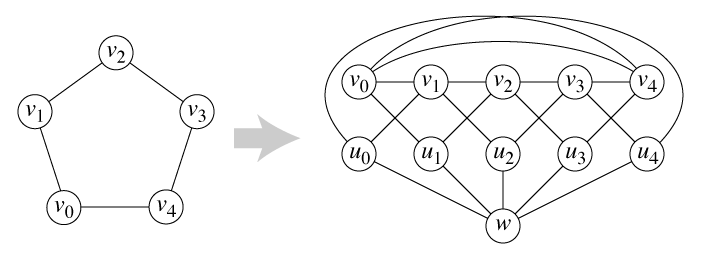
\includegraphics[width=\textwidth]{images/Groetzsch-as-Mycielski.png}
			\caption{Przykład transformacji Mycielskiego dla cyklu $C_{5}$}
		\end{center}
	\end{figure}

	W naszej analizie posłużyliśmy się mycielskianami od $M(3)$ do $M(7)$ i zbadaliśmy skuteczność naszych algorytmów na nich. Liczba chromatyczna mycielskianu $M(n)$ wynosi $n + 1$. 
	\\~\\
	Grafy Mycielskiego okazały się grupą grafów, dla której badane przez nas algorytmy działają najskuteczniej. Poza jednym przypadkiem (dla algorytmu AMIS dla grafu $M(7)$, każdemu grafowi udało się osiągnąć średnią niższą niż liczba chromatyczna.
	\\~\\
	Porównując badane algorytmy można stwierdzić, że nie ma jednoznacznie najlepszego algorytmu dla grafów Mycielskiego. Skuteczność algorytmu zależy zarówno od wielkości badanego grafu oraz liczby warstw, dla której szukamy naszego rozwiązania. Dla przykładu, dla grafu $M(3)$ najlepiej wypadły algorytmy AMIS i CS z wymianą - dla $p = 2$ współczynnik chromatyczny wynosił $3.5$ dla $100\%$ wywołań. Ogólnie rzecz ujmując, AMIS miał najlepsze wyniki spośród wszystkich algorytmów, w dodatku osiągając $100\%$ skuteczności. Nieco gorszy był CS z wymianą jednak nadal udawało się osiągać wyniki poniżej współczynnika $3.5$. Algorytmy DSATUR, pomimo nieco gorszych rezultatów, nadal były w stanie znaleźć dobre rozwiązania.
	\\~\\
	Wraz ze wzrostem $n$ widzimy zauważalny wzrost skuteczności, objawiający się różnicą między liczbą chromatyczną a współczynnikiem chromatycznym osiąganym przez testowane algorytmy. Można zauważyć, że algorytm AMIS, mimo zauważalnie gorszej skuteczności od pozostałych algorytmów w większości przypadków, jest w stanie osiągać 100\% skuteczność, co może być czynnikiem decydującym w przypadku konieczności użycia rozwiązania, które będzie dawać jednoznaczne rezultaty. Algorytm CS z wymianą w wielu przypadkach radził sobie najlepiej, jeśli chodzi o udział najbardziej optymalnych wyników w całości próby. Nie dawał jednak on tak dobrych rezultatów, jak niektóre iteracje algorytmu DSATUR, które bardzo często były lepsze od wzorcowej wartości liczby chromatycznej dla klasycznego przypadku nawet o $2$.
	\\~\\
	Nie można jednak stwierdzić bezpośrednio, który algorytm jest najlepszy. Przykładowo, dla $M(5)$ oraz liczby warstw $p=10$, mimo faktu, że algorytm AMIS na ogół dawał rezultaty gorsze od pozostałych algorytmów, w tym przypadku osiągałnajmniejszy współczynnik chromatyczny. Dla $M(7)$ oraz $p=5$ najlepszym wyborem powinien być algorytm DSATUR z wyborem po najniższej saturacji zewnętrznej, gdyż średni współczynnik chromatyczny był w tym przypadku najbardziej optymalny. Biorąc zaś pod uwagę graf $M(6)$ przy liczbie warstw $p = 3$, algorytm CS z wymianą dawał wartość $5.67$ dla 93\% obserwacji, co jest dobrym kompromisem między skutecznością a frekwencją występowań najlepszego rozwiązania.
	
	\begin{table}[H]
		\begin{minipage}{.5\linewidth}
			\centering
			\begin{tabular}{|l|c|c|c|c|}
				\hline
				\textbf{$p$} & \textbf{algorytm} & \textbf{$\min \chi_{p}$} & \textbf{$|\min \chi_{p}|$} & \textbf{$\overline{\chi_{p}}$} \\
				\hline
				2 & AMIS & 3.5 & 100 & 3.5 \\
				2 & interCS & 3.5 & 100 & 3.5 \\
				2 & oDSATUR & 3.5 & 48 & 3.76 \\
				2 & tDSATUR & 3.5 & 48 & 3.76 \\
				\hline
				3 & AMIS & 3.33 & 100 & 3.33 \\
				3 & interCS & 3.0 & 89 & 3.04 \\
				3 & oDSATUR & 3.67 & 48 & 3.84 \\
				3 & tDSATUR & 3.67 & 39 & 3.87 \\
				\hline
				5 & AMIS & 3.2 & 100 & 3.2 \\
				5 & interCS & 3.4 & 100 & 3.4 \\
				5 & oDSATUR & 3.4 & 2 & 3.82 \\
				5 & tDSATUR & 3.6 & 45 & 3.82 \\
				\hline
				10 & AMIS & 3.2 & 100 & 3.2 \\
				10 & interCS & 3.5 & 100 & 3.5 \\
				10 & oDSATUR & 3.3 & 3 & 3.73 \\
				10 & tDSATUR & 3.5 & 52 & 3.74 \\
				\hline
			\end{tabular}
			\caption{$M(3)$}
		\end{minipage}
		\begin{minipage}{.5\linewidth}
			\centering
			\begin{tabular}{|l|c|c|c|c|}
				\hline
				\textbf{$p$} & \textbf{algorytm} & \textbf{$\min \chi_{p}$} & \textbf{$|\min \chi_{p}|$} & \textbf{$\overline{\chi_{p}}$} \\
				\hline
				2 & AMIS & 4.5 & 100 & 4.5 \\
				2 & interCS & 4.5 & 100 & 4.5 \\
				2 & oDSATUR & 4.0 & 28 & 4.43 \\
				2 & tDSATUR & 4.0 & 29 & 4.46 \\
				\hline
				3 & AMIS & 4.33 & 100 & 4.33 \\
				3 & interCS & 4.0 & 91 & 4.03 \\
				3 & oDSATUR & 4.0 & 20 & 4.42 \\
				3 & tDSATUR & 4.0 & 6 & 4.57 \\
				\hline
				5 & AMIS & 4.0 & 100 & 4.0 \\
				5 & interCS & 4.4 & 100 & 4.4 \\
				5 & oDSATUR & 3.8 & 5 & 4.34 \\
				5 & tDSATUR & 4.0 & 2 & 4.52 \\
				\hline
				10 & AMIS & 3.7 & 100 & 3.7 \\
				10 & interCS & 4.5 & 100 & 4.5 \\
				10 & oDSATUR & 3.7 & 1 & 4.28 \\
				10 & tDSATUR & 4.0 & 20 & 4.45 \\
				\hline
			\end{tabular}
			\caption{$M(4)$}
		\end{minipage}
		\begin{minipage}{.5\linewidth}
			\centering
			\begin{tabular}{|l|c|c|c|c|}
				\hline
				\textbf{$p$} & \textbf{algorytm} & \textbf{$\min \chi_{p}$} & \textbf{$|\min \chi_{p}|$} & \textbf{$\overline{\chi_{p}}$} \\
				\hline
				2 & AMIS & 5.5 & 100 & 5.5 \\
				2 & interCS & 5.0 & 100 & 5.0 \\
				2 & oDSATUR & 4.5 & 12 & 5.08 \\
				2 & tDSATUR & 4.5 & 16 & 5.14 \\
				\hline
				3 & AMIS & 5.67 & 100 & 5.67 \\
				3 & interCS & 4.67 & 2 & 5.01 \\
				3 & oDSATUR & 4.33 & 1 & 5.06 \\
				3 & tDSATUR & 4.67 & 3 & 5.3 \\
				\hline
				5 & AMIS & 5.4 & 100 & 5.4 \\
				5 & interCS & 5.0 & 100 & 5.0 \\
				5 & oDSATUR & 4.2 & 1 & 4.94 \\
				5 & tDSATUR & 4.8 & 6 & 5.22 \\
				\hline
				10 & AMIS & 4.7 & 100 & 4.7 \\
				10 & interCS & 5.0 & 100 & 5.0 \\
				10 & oDSATUR & 4.3 & 1 & 4.8 \\
				10 & tDSATUR & 4.5 & 5 & 5.14 \\
				\hline
			\end{tabular}
			\caption{$M(5)$}
		\end{minipage}
		\begin{minipage}{.5\linewidth}
			\centering
			\begin{tabular}{|l|c|c|c|c|}
				\hline
				\textbf{$p$} & \textbf{algorytm} & \textbf{$\min \chi_{p}$} & \textbf{$|\min \chi_{p}|$} & \textbf{$\overline{\chi_{p}}$} \\
				\hline
				2 & AMIS & 6.0 & 100 & 6.0 \\
				2 & interCS & 6.0 & 100 & 6.0 \\
				2 & oDSATUR & 5.0 & 4 & 5.79 \\
				2 & tDSATUR & 5.0 & 10 & 5.7 \\
				\hline
				3 & AMIS & 6.67 & 100 & 6.67 \\
				3 & interCS & 5.67 & 93 & 5.69 \\
				3 & oDSATUR & 5.0 & 3 & 5.65 \\
				3 & tDSATUR & 5.0 & 2 & 5.91 \\
				\hline
				5 & AMIS & 6.6 & 100 & 6.6 \\
				5 & interCS & 5.8 & 100 & 5.8 \\
				5 & oDSATUR & 5.0 & 9 & 5.45 \\
				5 & tDSATUR & 5.2 & 2 & 5.89 \\
				\hline
				10 & AMIS & 5.9 & 100 & 5.9 \\
				10 & interCS & 6.0 & 100 & 6.0 \\
				10 & oDSATUR & 4.9 & 4 & 5.37 \\
				10 & tDSATUR & 5.1 & 1 & 5.81 \\
				\hline
			\end{tabular}
			\caption{$M(6)$}
		\end{minipage}
		\begin{minipage}{\linewidth}
			\centering
			\begin{tabular}{|l|c|c|c|c|}
				\hline
				\textbf{$p$} & \textbf{algorytm} & \textbf{$\min \chi_{p}$} & \textbf{$|\min \chi_{p}|$} & \textbf{$\overline{\chi_{p}}$} \\
				\hline
				2 & AMIS & 8.0 & 100 & 8.0 \\
				2 & interCS & 7.0 & 100 & 7.0 \\
				2 & oDSATUR & 5.5 & 4 & 6.35 \\
				2 & tDSATUR & 5.5 & 1 & 6.32 \\
				\hline
				3 & AMIS & 7.67 & 100 & 7.67 \\
				3 & interCS & 6.33 & 94 & 6.35 \\
				3 & oDSATUR & 5.67 & 16 & 6.15 \\
				3 & tDSATUR & 5.67 & 1 & 6.53 \\
				\hline
				5 & AMIS & 7.6 & 100 & 7.6 \\
				5 & interCS & 7.0 & 100 & 7.0 \\
				5 & oDSATUR & 5.4 & 1 & 6.05 \\
				5 & tDSATUR & 6.0 & 1 & 6.55 \\
				\hline
				10 & AMIS & 6.9 & 100 & 6.9 \\
				10 & interCS & 7.0 & 100 & 7.0 \\
				10 & oDSATUR & 5.3 & 1 & 5.88 \\
				10 & tDSATUR & 5.8 & 1 & 6.49 \\
				\hline
			\end{tabular}
			\caption{$M(7)$}
		\end{minipage}
		\caption{Porównanie współczynników chromatycznych osiąganych przez testowane algorytmy na grafach Mycielskiego dla wybranych ilości warstw }
	\end{table}
	
	\section{Wnioski końcowe}
	
	Kolorowanie warstwowe nie daje rezultatów lepszych od klasycznego kolorowania dla wszystkich grafów. Istnieją jednak grafy, dla które na pewno posiadają taką własność. Do takich grafów, poza nieparzystymi cyklami, można zaliczyć na pewno niektóre grafy Knesera (w szczególności takie, dla których $n > 2k + 1$) czy grafy Mycielskiego. Niemniej jednak, dla większości grafów problem znalezienia pokolorowania warstwowego lepszego od klasycznego jest trudny do rozwiązania.
	\\~\\
	Ilość warstw $p$ w problemie ma znaczący wpływ na wartość współczynnika $p$-chromatycznego. W większości badanych przypadków większa ilość warstw wiązała się z mniejszym współczynnikiem chromatycznym. Mamy bowiem więcej możliwości tasowania kolorami w taki sposób, aby uzyskać mniejszą liczbę kolorów w naszym kolorowaniu. 
	\\~\\
	Algorytm AMIS w większości przypadków dawał gorsze pokolorowania, jednakże gdy udało mu się takie znajdować, zazwyczaj był konsekwentny i dla wszystkich przypadków zwracał pokolorowanie lepsze od klasycznego. Algorytmom z rodziny DSATUR udawało się znajdować najlepsze rozwiązania rzadziej, jednakże stanowiły one mały odsetek całej próby. W ogólnym rozrachunku średnie wyniki najczęściej (chociaż nie zawsze) były gorsze od algorytmu CS z wymianą. Trudno tutaj rozróżnić wersję z sortowaniem względem całkowitej saturacji od wersji z sortowaniem po zewnętrznej saturacji, jednak wersja z zewnętrzną saturacją wydaje się nieco skuteczniejsza. 
	\\~\\
	Algorytm CS z wymianą koloru wierzchołka wydaje się kompromisem między jakością a ilością. Nie znajdował on najmniejszego możliwego pokolorowania, jednakże często znaczną część próby stanowiły pokolorowania lepsze od klasycznego (gdy działał on skutecznie). Jednakże, algorytm CS z wymianą działał zdecydowanie najdłużej ze wszystkich. Algorytm AMIS działał znacznie krócej od poprzednika, jednak faworytem są tutaj algorytmy DSATUR. Ich czas działania był najkrótszy, z niewielką przewagą algorytmu sortującego po saturacji zewnętrznej (co wynika z faktu, że odchodzi nam konieczność dodawania saturacji zewnętrznej i wewnętrznej przy liczeniu saturacji całkowitej).
	\\~\\
	Problem kolorowania warstwowego ma swoje realne zastosowania w postaci m.in. alokacji większej ilości zasobów do danych urządzeń czy alokacji zadań do wybranych podmiotów. W przypadku, gdy graf problemu da się pokolorować lepiej niż klasycznie, aplikacja skutecznych algorytmów aproksymacyjnych może usprawnić działanie wielu procesów. 
	
	\vspace*{\fill}
	
	\begin{thebibliography}{0}
		\bibitem{kubale-article}
		Marek Kubale, \textit{Analiza efektywności algorytmów kolorowania grafów}, PTM 1980\\
		\url{https://wydawnictwa.ptm.org.pl/index.php/matematyka-stosowana/article/viewFile/1531/1457}\\
		\textit{(dostęp: \today)}
		
		\bibitem{kubale-book}
		Marek Kubale, \textit{Optymalizacja dyskretna. Modele i metody kolorownia grafów}, WNT 2002
		
		\bibitem{radin-thesis}
		Andrew Radin, \textit{Graph coloring heuristics from investigation ofsmallest hard to color graphs}, RIT Scholar Works 2000
		\url{http://citeseerx.ist.psu.edu/viewdoc/download?doi=10.1.1.867.178\&rep=rep1\&type=pdf}
		\textit{(dostęp: \today)}
		
		\bibitem{gci}
		\url{https://mat.tepper.cmu.edu/COLOR/instances.html#XXCUL}
		\textit{(dostęp: \today)}
		
		\bibitem{mycielskian}
		\url{https://en.wikipedia.org/wiki/Mycielskian}
		\textit{(dostęp: \today)}
		
		
	\end{thebibliography}
	

\end{document}